\documentclass[french, english]{article}
\usepackage[utf8]{inputenc}
\usepackage[T1]{fontenc}
\usepackage[french, english]{babel}

\usepackage{graphicx}
\usepackage{multicol}
\setlength{\columnsep}{5cm}
\usepackage{hyperref}
\usepackage{nameref}
\usepackage{textcomp}
\usepackage{gensymb}
\newcommand{\hsp}{\hspace{20pt}}
\newcommand{\HRule}{\rule{\linewidth}{0.5mm}} 
\usepackage{float}
\usepackage{geometry}
\usepackage{ccaption}
\usepackage{amsmath}
\usepackage{amssymb}
\usepackage{textcomp}
\usepackage{mathabx}
\usepackage{stmaryrd}
\usepackage{verbatim}
\newcommand{\etal}{\textit{et al}., }

%\geometry{top=3cm, bottom=3cm, left=2cm, right=2cm}


\begin{document}


%%%%%%%%%%%%%%%%%
% PAGE DE GARDE %
%%%%%%%%%%%%%%%%%

\title{Analyse pyramidales d'images globale avec une architecture U-Net hautement supervisée}

%\author{First Author\\
%Institution1\\
%Institution1 address\\
%{\tt\small firstauthor@i1.org}

\author{
Michele BONA \quad Clémence Gaillotte \quad Tristan Michel \quad Damien Djomby \quad Enzo Masson\\
Ecole de Technologie Supérieur\\
{\tt\small \{michele.bona.1, clemence.gaillotte.1, tristan.michel.1, damien.djomby.1, enzo.masson.1\}@ens.etsmtl.ca}}
\date{Décembre 2021}

\maketitle

\normalsize

%\selectlanguage{english}
\begin{abstract}
In this paper we present SubUNet, a new architecture for medical image segmentation (MRIs). Our model is inspired by the UNet architecture and adds the Pyramid Pooling Module (PPM) of the PSPNet architecture. The addition of this module serves mainly to add a global observation of our image by increasing the receptive field of the model in order to detect the various parts of the heart by their shape and according to the organs which surround it. Thus, by combining the precision of Unet for the details of the images and the PPM we manage to detect the right ventricle, the left ventricle and the myocard on MRIs of hearts with a better precision than UNet.
\end{abstract}

\selectlanguage{french}
\begin{abstract}
Dans ce papier nous présentons SubUNet, une nouvelle architecture pour la segmentation d'images médicales (IRMs). Notre modèle s'inspire de l'architecture de UNet et ajoute le Pyramid Pooling Module (PPM) de l'architecture PSPNet. L'ajout de ce module sert principalement à ajouter une observation globale de notre image et d'augmenter le champ réceptif de notre modèle afin de pouvoir détecter les différentes parties du coeur par leur forme et en fonction des organes qui les entourent. Ainsi, en combinant la précision de UNet pour les détails des images et le PPM nous arrivons à détecter le ventricule droit, le ventricule gauche et la myocarde sur des IRMs de coeurs avec une meilleure précision que UNet.
\end{abstract}


\section{Introduction}  

\subsection{Problématiques}
\paragraph{}Lors de ces dernières décennies, l'imagerie par résonance magnétique (IRM) est devenue un examen essentiel pour l'étude du coeur humain. Cependant, en raison des caractéristiques des images IRM cardiaques et de la grande variabilité des images entre les patients, le problème de l'identification automatique des différentes parties du coeur dans les IRMs s'est posé et est toujours très étudié.
\paragraph{} D'un autre côté la recherche concernant le traitement d'images par des réseaux de neurones avance de plus en plus vite, et le sujet de la segmentation automatiques des IRMs avance avec elle. Ainsi on peut se demander comment identifier automatiquement sur des IRMs de coeurs humains le ventricule droit, le ventricule gauche et la myocarde. 
\paragraph{} Ce type de segmentation demande des connaissances techniques concernant le coeur humain, et le développement d'un réseau de neurones la faisant automatiquement permettrait d'aider à l'analyse des IRMs et d'accélérer les diagnostics des médecins. 


\subsection{Contributions}
\paragraph{} Comme nous allons voir dans la section \nameref{method}, nous nous sommes inspiré des réseaux de neurones les plus efficaces et utilisés, particulièrement U-Net. Après les avoir implémentés et avoir créé notre modèle nous avons remarqué que nous avions une meilleure segmentation que U-Net, et une précision très satisfaisante pour la segmentation du ventricule droit qui pose en généralement le plus de problèmes sur ce jeu de données.


\section{État de l'art}

\paragraph{}L'apprentissage automatique est aujourd'hui au centre de beaucoup de sujets de recherche sur l'imagerie médicale en raison de son importance et des progrès importants que cela pourrait apporter dans le milieu médical. C'est donc l'objet de nombreux challenges d'apprentissage automatique, qui permettent à des chercheurs de proposer des modèles de plus en plus performants pour ces challenges.

\subsection{Méthodes de segmentation d'imagerie médicale}

\paragraph{}Il existe notamment beaucoup de modèles répondant aux problèmes de la segmentation d'imagerie médicale et nous allons nous concentrer sur quelques modèles et fonctions de coûts s'étant démarqués des autres.

%U-net
\subsection{U-Net}
\paragraph{} C'est le cas du réseau U-Net connu pour son architecture en forme de U, composé d'une partie "encodeur" et d'une partie "décodeur".Il s'agit d'un réseau entièrement convolutif qui est basé sur un réseau fully connected (FCN)\paragraph{}

U-Net a été créé par \emph{Olaf Ronneberger, Philipp Fischer et Thomas Brox} en 2015 dans le cadre de leur participation et victoire au challenge ISBI (challenge de segmentation pour l'imagerie médicale) en Novembre 2015. Le score de leur modèle a dépassé de plus de 10\% les scores des autres modèles. Le réseau U-net a été présenté plus explicitement dans leur papier \emph{U-Net: Convolutional Networks for Biomedical Image Segmentation} \cite{UNet}. Depuis le réseau a été repris et légèrement modifié par de nombreuses équipes dans le cadre de la segmentation pour l'imagerie médicale.

En 2018, le réseau U-Net++ \cite{U-Net++} conserve le principe d'un sous-réseau d'encodage puis d'un sous-réseau de décodage, une des principales modifications et la liaison entre ces deux sous réseaux avec des Skip connections ainsi qu'un usage de la supervision profonde.

Enfin en 2021, le réseau GA-Unet \cite{GA-UNet} est créé. Le modèle utilise le réseau de neuronne convolutionnel VGG16 comme encodeur du réseau U-Net. Les couches de pooling présentes dans U-Net sont remplacées par des opéarations d'Upsamplings. 

\subsection{PSPNet} Le réseau PSPNet a été créé en 2016 \cite{PSPNet} dans le cadre d'un challenge de segmentation. Ce réseau n'est pas spécialement prévu pour l'imagerie médicale mais il obtient des résultats très performant pour la segmentation. \paragraph{}Ce réseau est composé d'une architecture encodeur-décodeur et contient des pyramid pooling modules (PPM). Ces modules permettent de donner un contexte global a l'image avant de faire une prédiction locale. Il s'agit d'une amélioration par rapport a ResNet \cite{ResNet} qui est un modèle ayant rencontré des difficultés à capturer le contexte global d'un image malgré un champ réceptif en entrée très grand.


\subsection{Fonctions de coûts}
Il existe de nombreuses fonctions de coûts mais certaines ont particulièrement démontrés leur efficacité dans les problème de segmentation d'imagerie médicale. Il existe la cross-entropie qui est très souvent utilisée. Cette fonction de coût fonctionne au niveau du pixel et est la base de nombreuses autres fonctions de coûts.
\paragraph{}Une fonction de coût régulièrement utilisé en segmentation d'imagerie médicale est la Dice loss. Cette fonction permet de calculer la similarité entre deux images et permet une meilleure définition des contours. 
\paragraph{}Enfin il existe la Focal Loss introduite dans le cadre de la détection d'objets denses \cite{Focal-Loss}. Il s'agit d'une variation de la Cross-entropie qui permet de mettre plus de poids sur les exemples ayant été difficilement classés et qui fonctionne très bien même si les classes ne sont pas équilibrées. Cette fonction de coût a généralement un bonne impact sur la vitesse de convergence.


\paragraph{}



\section{Méthode}
\label{method}

\subsection{Données d'entraînement}
Nos données d'entraînement sont 1208 images différentes d'IRMs de coeur sur différents patients (et 90 images de validation). Les images montrent un coeur selon différentes coupes transversales, toutes en différents niveaux de gris et de taille 256x256. 
Le seul pré-traitement que nous avons appliqué est d'équilibrer l'histogramme de niveau de gris des images.

\subsection{Augmentation de données}

Le corps humains est complexe et il y a une grande variabilité des placements et de la taille des organes.
Cela se voit particulièrement lorsque l'on essaye de faire de la segmentation d'images de coeurs humain pour en extraire les différentes parties.\\
% Nous avons peu de données et ces données sont vraiment différentes les unes des autres.
% Nous avons donc chercher à prévoir la variabilité que peut nous amener différentes prises d'IRMs, par exemple dans certains cas certaines classes ne sont pas présentes.
Afin d'éviter l'over-fitting sur notre petit jeu de données, nous avons mis en place une augmentation de données (Data Augmentation, en anglais) qui reste cohérente avec les possibilités que nous pouvons rencontrer dans le monde.
Pour cela il a fallu prendre en compte différentes malformations qui peuvent atteindre les patients.
Nous avons donc une dizaine de transformations possible, chacune avec une probabilité de 0.2 de s'appliquer. Cette valeur élevé permet d'entraîner notre modèle sur des données très variées.
Les transformations possibles sont:

\begin{list}{\textbullet}{}
 \item un vertical flip (mirroir sur l'axe horizontal)
 \item un mirror horizontal flip
 \item une rotation avec un angle allant de -30° à 30° choisi aléatoirement
 \item un crop (Zoom), la taille du sous-cadre vaut entre 0 et 1/2 taille du cadre original, la position du sous-cadre dépend d'un bord choisi aléatoirement
 \item un padding (Ajout d'une marge noire)
 \item un z shift
 \item un brightness shift (changement de luminosité)
 \item un flou gaussien (qui nous a été très utile)
 \item un auto-contrast
 \item un changement de sharpness (d'une valeur entre 0 et 2)
\end{list}

% Ces transformations sont appliquées à l'aide de la bibliothèque Torchvision de Pytorch. 

\subsection{Choix du modèle}
\paragraph{}Empiriquement, la recherche a largement prouvé que la structure UNet est l'une des plus efficaces pour la segmentation d'imagerie médicale.
Pour conserver la taille de nos images d'entré pour la sortie du modèle, nous avons choisi d'ajouter un padding pour les convolutions, au lieu de faire un padding mirroir sur toutes nos images comme présenté par Ronneberger \etal\cite{UNet}. 
Et cela évite le zoom naturellement présent entre les features maps que on retrouve dans UNet, en effet nous ne voulions pas perdre des informations (même si ce n'est que certains pixels sur les bords, car cela pourrait être décisif pour reconnaître les différentes parties du coeur).\\

\paragraph{}Suite à nos expérimentations nous avons des meilleurs résultats avec les modèles de UNet et de PSPNet (grâce au Pyramid Pooling Module). Ces résultat sont parfaitement cohérent car UNet est le meilleur pour la segmentation médicale, donc son encodeur et son décodeur sont excellent. 
De plus le module PPM de PSPNet permet d'avoir un context plus global dans notre détection et ainsi essayer de repérer des formes qui entour le coeur (par exemple situer le coeur par rapport aux poumons).
Nous avons ajouté des modules Deeply-Supervised dans le décodeur de UNet pour essayer de controler l'apprentissage dans la bonne direction mais malheureusement leur efficacité n'est pas concluante, comme nous le présenterons dans la section \ref{robustesse}.
\paragraph{}Ainsi en combinant l'encodeur et le décodeur de UNet avec le PPM de PSPNet nous devrions avoir un modèle capable de faire une segmentation précise (avec les skip connections de UNet).
Le tout en se basant sur une observation globale de notre image afin de pouvoir détecter les différentes parties du coeur par leur forme et en fonction des organes qui l'entoure.
De plus d'après l'état de l'art et de nos expérimentations, nous avons utilisé des Average Poolings au lieux de Max Poolings dans l'encodeur UNet car cela fonctionne mieux par la suite avec le module PPM. La section \ref{robustesse} présente aussi les aventage de Avg Pooling.
Ce modèle, présenté en figure \ref{model},  permet donc une segmentation avec cohérence d'environnement en prenant les avantages de UNet et du PPM.

\begin{figure}[!t]
    \centering
    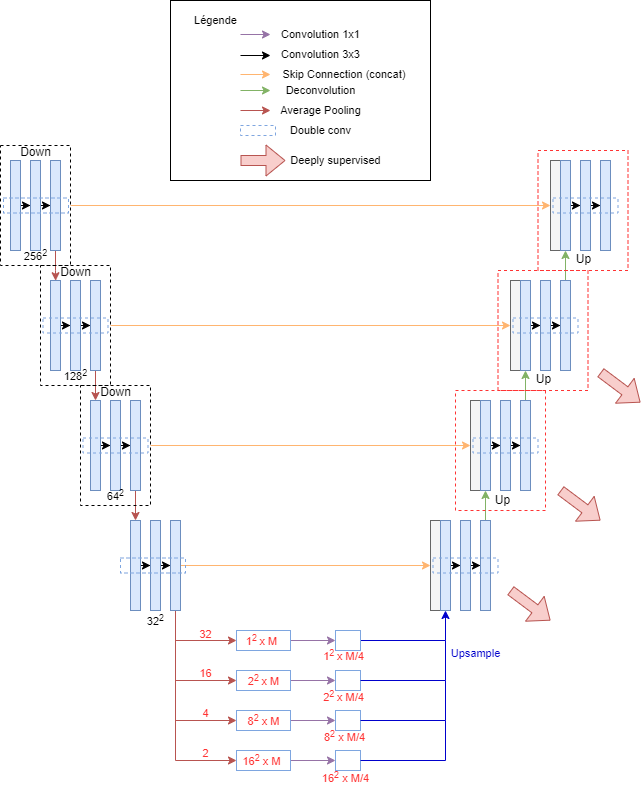
\includegraphics[scale=0.45]{img/SubUnetAvecPPM.png}
    \caption{Architecture de notre modèle, basée sur un encodeur et un décodeur UNet avec Average pooling et dé-convolution, et un pyramidal pooling module.}
    \label{model}
\end{figure}

\subsection{Entraînement du réseau}
\label{training}

\paragraph{}Nous avons entraîné notre modèle avec une taille de batch de 56 images. Nos recherches ont montré qu'un grand nombre d'images par batch donnait de meilleurs résultats. Pour la mis-à-jour de nos paramètres nous avons choisi d'utiliser la politique de `poly' taux d'apprentissage où le taux d'apprentissage de l'epoch est égale au taux d'apprentissage de départ de \(3,15\times 10^{-4}\) multiplié par $(1-\frac{iter}{max_iter})^{power}$. Pour la valeur de la puissance, nous avons pris la même valeur que celle présenté dans le papier de PSPNet, soit \(0,9\). Concernant la fonction de coût, nous avons utilisé une combinaison du coefficient de Dice et de Focal loss \(loss(X,Y) = \alpha \cdot FocalLoss_{\gamma}(X,Y)+(1-\alpha) \cdot DiceLoss(X,Y)\), avec \(\alpha=0,233\) et \(\gamma=1,977\).

\paragraph{}Inspiré par Ye \etal\cite{multidepth_fusion}, nos branches profondément supervisées sont une successions de Convolution transposée 2D permettant de remonté à la taille d'origine de l'image d'entrée. Nous calculons ensuite l'erreur de chaque prédiction (branches principale et supervisées) par rapport à la vérité terrain et nous sommons ensuite ces erreurs. La rétro-propagation est calculé à partir de ce résultat et propagé à tous le modèle.

% \begin{comment}
% Dans un premier temps nous nous sommes occupés de l'aspect matériel. Nous avons donc chargé nos données Compute Canada et nous nous sommes connecté à Narval, situé à l'ETS. Nous avons ensuite dû réservé des ressources pour notre projet. Afin d'être bien placé sur la liste d'attente à chaque fois que nous avions besoin de réaliser des calculs, nous avons tenté de réserver le minimum de ressources possibles. Nous avons donc demandé un noeud avec carte graphique et un coeur de processeur seulement.

% On a chargé nos données sur compute canada connecté sur Narval à l'Éts, nous avons reservé un noeud avec une carte graphique, un unique coeur de processeur, on réserve le minimum possible pour qu'on nous attribut un noeud plus vite (si tu demandes moins c'est plus facilement disponible), on prenais noeud avec carte graphique nvidia A100 (un noeud = un entrainement sur 1 carte graphique) ducoup les tests sur des noeuds en parallèles (jusqu'à 100 en meme temps). \\
% Carte A100 a beaucoup de V-Ram (40Go), c'est la mémoire, ducoup permet de stocker beaucoup de choses COMME les résultats (car si on stocke sur carte c'est plus rapide, pas besoin de upload ou download les données). Donc on a chargé tout le dataset sur la carte. POur charger sur noeud on chargeait images sous forme de tensor (pour faire les calculs direct, c'est des matrices, calculs groupés et plus rapide, facilite calculs). Charge tout sur la carte car si on charge des batchs, quand on les transforme on les perd après pour charger un autre batch, là \textbf{on a accès à tout direct} \\
% \end{comment}


%\subsection{Optimisation des hyperparamètres}

% Nous avons créé une environnement complet pour l'implémentation  et le test de modèles de segmentation médicale. Nous avons donc de nombreux hyperparamètres à optimiser comme par exemple le batch size ou encore le taux d'apprentissage. nous avons donc entrainé notre modèle puis optimisé ces hyperparamètres.

% \begin{comment}
% \begin{figure}[H]
%     \centering
%     \includegraphics[scale=0.45]{img/parametresTraining.png}
% \end{figure}
% \end{comment}

%Pour avoir le meilleur modèle pour le test final, nous avons procédé à une optimisation des hyperparamètres. Cette optimisation à eu lieu en deux parties, premièrement nous avons optimisé les paramètres discrets avec un algorithme de Grid Search. Puis pour les hyperparamètres restant qui étaient continu nous avons fait un Random Search. Pour pouvoir optimiser correctement nos paramètres discret, nous basons la valeur de nos paramètres continus sur l'état de l'art.\\
%Les hyperparamètres discrets sont les suivants:
%\begin{list}{\textbullet}{}
%    \item Les paramètres du modèle à entraîner
%    \item Les fonctions de loss
%    \item Les optimisateurs
%\end{list}
%Les paramètres du modèle à entraîner sont l'ensembles des choix de notre architecture du réseau que nous voulons faire varier pour trouver le meilleur modèle.
%Soit l'inclusion ou non des modules Deeply-Supervised et l'utilisation de Max Pooling ou de Average Pooling.\\

%Il existe deux types de fonction de perte : les fonctions "ensemblistes" et les fonctions "par pixel". Lorsque nous avons réalisés le GridSearch, nous avons donc testé chaque fonction et combinaison de fonctions ensemblistes et par pixel. Les fonctions de mêmes types sont corrélés, c'est pour cette raison que nous n'avons pas trouvé pertinent de combiner deux fonctions du même type.\\

%Enfin pour optimiser les autres hyperparamètres, nous réalisons un RandomSearch. Les hyperparamètres sont choisis aléatoirement sur 100 jobs, et seuls ceux du meilleur job sont gardés.\\
%Ces paramètres sont:
%\begin{list}{\textbullet}{}
%    \item Le batch size, aléatoirement choisi suivant une loi uniforme dans $[0,50]$
%    \item La learning rate, choisit avec une loi exponentielle dans $[0,1]$
%    \item $\gamma$, valeur utilisé dans les fonctions de loss focal qui suit une loi uniforme dans $[0,4]$
%    \item $\alpha$, coefficient de combinaison entre nos deux fonctions de loss, suit une loi uniforme %qui varie dans $[0,1]$\\
%    Exemple avec Focal Loss et Dice loss :
%    \begin{equation*}
%        loss(X,Y) = \alpha \cdot FocalLoss_{\gamma}(X,Y)+(1-\alpha) \cdot DiceLoss(X,Y)
%    \end{equation*}
%\end{list}


\section{Résultats}

\subsection{Résultats sur le challenge}
\paragraph{Comparatif aux autres modèles}
\label{comp:models}
Lors de nos recherches préalables, nous avons effectué un grid search afin de déterminer quels étaient les modèles et les fonctions de coût les plus prometteurs pour le défi de segmentation. Nous avons implémenté les modèles SegNet, PSPNet (avec un simple encodeur au lieu de ResNet), UNet ainsi qu'une adapation de VGG permettant la segmentation. Nous avons aussi étudier différentes fonctions de coût dont les recherches et les résultats seront présenté dans la section \nameref{loss_ablation}. Le tableau \ref{tab:baseline} présente les résultats obtenus pour ce gridsearch. Sans surprises, UNet arrive en première position mais PSPNet donne aussi de bon résultats alors que ce dernier avec été implémenté avec un encodeur et un décodeur beaucoup plus simple que celui décris par Zhao \etal\cite{PSPNet}. Ainsi nous est venu l'idée d'utiliser le Pyramid Pooling Module au sein d'un UNet.

\begin{table}[h]
    \centering
    \footnotesize
    \begin{tabular}{l l c c c}
        \hline
        Modèle & Fonction de coût & Mean IoU(\%) & Mean Dice(\%) & Mean Soft Dice(\%)\\
        \hline
        \hline
        VGG & focal tversky loss + focal loss & 65,92 & 77,81 & 19,55\\
        SegNet & jaccard loss + focal loss & 77,18 & 86,33 & 19,37\\
        \textit{PSPNet} & ce loss & \textit{79,44} & \textit{87,86} & \textit{20,35}\\
        \textbf{UNet} & jaccard loss & \textbf{85,52} & \textbf{92,01} & \textbf{92,29}\\
        \hline
    \end{tabular}
    \caption{Meilleurs résultats obtenus après le grids earch pour chaque modèle, spécifiant la fonction de coût ayant donné ces meilleurs résultats.}
    \label{tab:baseline}
\end{table}

% grid search
\paragraph{Vitesse de convergence}
Comme nous pouvons le voir sur la figure \ref{fig:convergence}, SubUNet converge plus vite que UNet lorqu'il est entrainé avec notre module profondément supervisé. Néanmoins, la section \ref{robustesse} montrera que nous avons obtenus de meilleurs résultat sans ce module mais avec une vitesse de convergence plus faible.

\begin{figure}[h]
    \centering
    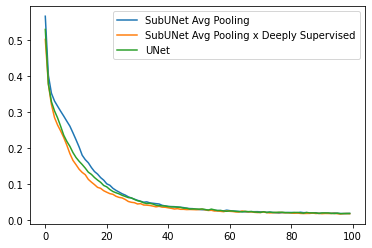
\includegraphics[scale=0.5]{img/convergence.png}
    \caption{Comparaison des convergence de la fonction de coût sur le dataset d'entraînement pour notre baseline et notre modèle avec et sans module profondément supervisé.}
    \label{fig:convergence}
\end{figure}


\paragraph{Améliorations visuelles}
Comme le montre la figure \ref{fig:baseline}, notre modèle permet une meilleur prédiction du ventricule droit qui est, selon nous, la classe la plus dure à prédire. Puisqu'elle peut aussi être la classe prépondérante sur certaines images, cette dernière peut baisser de façon considérable le score d'un modèle ayant du mal à généraliser. Nous remarquons que UNet a plus de mal a prédire le ventricule droit. Ce problème de prédiction sur le ventricule droit avec UNet est un problème que nous avons indentifié dés le début du challenge et est le principal point que nous avons essayer de résoudre. Ainsi, à l'issue de nos recherches, le modèle proposé a généralement une prédiction plus proche de la ground truth pour ce ventricule.

\begin{figure}[h]
    \centering
    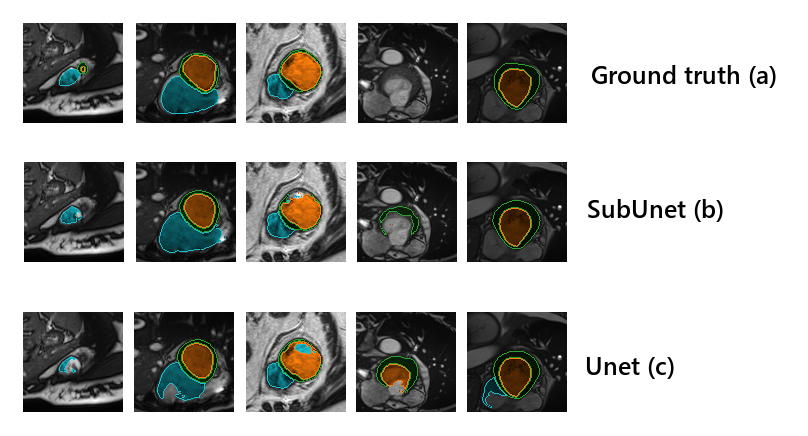
\includegraphics[scale=1.75]{img/comparaison.png}
    \caption{Amélioration visuelles sur le dataset de notre modèle (b) comparé à notre baseline(c). Ce figuré présentre le ventricule gauche en \textit{orange}, la myocarde du ventricule gauche en \textit{vert} et le ventricule droit en \textit{bleu}. Les deux modèles, SubUNet et notres baseline ont été entraîné dans les mêmes conditions.}
    \label{fig:baseline}
\end{figure}




\subsection{Étude de la robustesse de notre méthode}
\label{robustesse}

\paragraph{Étude d'ablation pour SubUNet} Pour étudier les performances de notre modèle, comparé à notre baseline, nous avons effectué différents entraînements avec différentes configurations, notamment le type de pooling utilisé et l'usage ou non de notre module profondément supervisé. Comme listé dans le tableau \ref{tab:ablation:model}, l'average pooling fonctionne mieux que le max pooling, ce qui rejoint les résultats obtenus par Zhao \etal\cite{PSPNet}. On remarque aussi que notre module profondément supervisé n'a pas donné de si bons résultats, ce qui peut s'expliquer par une mauvaise implémentions de notre part ou que envoyons un gradient trop fort sur les branches annexes, baissant ainsi la précision dans la branche principale.
\begin{table}[H]
    \footnotesize
    \centering
    \begin{tabular}{ l c c c }
        \hline
        Method & Mean IoU(\%) & Mean Dice(\%) & Mean Soft Dice(\%) \\
        \hline\hline
        %FCN \cite{long2015fully} & 29.39 & 71.32 \\
        PSPNet & 79,62 & 88,20 & 90,50 \\
        UNet & 84,77 & 91,49 & 93,10 \\
        SubUNet MP & 85,10 & 91,75 & 93,41 \\
        SubUNet MP x Deeply Supervised & 85,13 & 91,78 & 93,31 \\
        SubUNet AP x Deeply Supervised & 85,50 & 92,02 & 93,58 \\
        \textbf{SubUNet AP} & \textbf{85,63} & \textbf{92,06} & \textbf{93,65} \\
        \hline
    \end{tabular}
    \caption{Étude de notre modèle selon différents paramètres. `MP' et `AP' signifient respectivement   `Max Pooling' et `Average Pooling' et `DP' correspond à notre module de supervision profonde. Nos résultats ont été obtenus sur le jeu de données de validation après un entraînement avec nos meilleurs hyperparamètres (détaillés en section \ref{hyperparameters}) et avec augmentation de données sur 400 epochs.}
    \label{tab:ablation:model}
\end{table}

\paragraph{Étude d'ablation pour la fonction de coût hybride}
\label{loss_ablation}
Comme décrit dans la section \ref{comp:models}, nous avons effectué un gridsearch pour étudier quelles fonctions de coût et quels modèles baseline donnaient les meilleurs résultats. Nous avons donc pu déterminer que pour ce challenge, le couple \(Dice Loss + Focal Loss\) permettaient une très bonne performance. L'idée principale était de voir si la combinaison d'une fonction de coût dites `ensembliste' (qui compare la prédiction et la vérité terrain comme des ensemble) et d'une fonction de coût pixel à pixel (pixel-wise) donnerait de meilleurs résultats. Le résultat de ce gridsearch était évident, une combinaison donne généralement de légèrement meilleurs résultats. Le tableau \ref{tab:ablation:loss} présente les résultats obtenus par ablation sur la fonction de coût \(Dice + Focal\) avec notre modèle SubUNet.

\begin{table}[H]
    \footnotesize
    \centering
    \begin{tabular}{ l c c c }
        \hline
        Method & Mean IoU(\%) & Mean Dice(\%) & Mean Soft Dice(\%) \\
        \hline\hline
        Focal loss & 81,29 & 89,17 & 90,39 \\
        Dice loss & 85,59 & 91,78 & 93,32 \\
        \textbf{Dice loss + Focal loss} & \textbf{85,75} & \textbf{92,08} & \textbf{93,68} \\
        \hline
    \end{tabular}
    \caption{Étude par ablation des fonctions de coût utilisées. Nos résultats on été obtenus sur notre modèle SubUnet avec nos meilleurs hyperparamètres et augmentation de données sur  200 epochs. La combinaison \(Dice + Focal\) a été obtenue avec un \(\alpha=0,5\). La section \ref{hyperparameters} présente la valeur optimale que nous avons obtenu pour ce paramètre.}
    \label{tab:ablation:loss}
\end{table}

\paragraph{Hyperparamètres}
\label{hyperparameters}
Pour déterminer les hyperparamètres de notre modèle, nous avons effectué un random search sur les paramètres suivants : la taille de batch, le \(\alpha\) et le \(\gamma\) de notre fonction de coût présenté dans la section \nameref{training} ainsi que le taux d'apprentissage. Pour notre random search, nous avons effectué 200 entraînements de 400 epochs chacun, le taux d'apprentissage a été tiré selon une distribution normale puis a été amené à la puissance 5 pour obtenir de petites valeurs. Soit \(r\) une valeur aléatoire entre 0 et 1, \(lr = r^5\). Le tableau \ref{tab:comp_params} présente les résultats de cette recherche et les meilleurs paramètres que nous avons obtenu et utilisé pour l'entraînement de nos modèles. Néanmoins il semblerait que des batchs encore plus grand auraient pu donner de meilleurs résultat mais nous nous sommes retrouvé face à un problème technologique : au-delà de 60 images par batchs, nous arrivions à la limite de RAM de nos cartes graphiques (nos modèles ont été entraîné sur une carte Nvidia A100 40Go par entraînement).

\begin{table}[H]
    \footnotesize
    \centering
    \begin{tabular}{c c c c c c c}
        \hline
        Batch & \(\alpha\) & \(\gamma\) & lr & mean iou(\%) & mean dice(\%) & mean soft dice(\%)\\
        \hline
        \hline
        \([1;100]\) & \([0;1]\) & \([0;4]\) & \([0;1]\) \\
        \hline
        63 & 0,054 & 1,351 & \(1,52\times 10^{-2}\) & 87,53 & 93,24 & 94,70\\
        67 & 0,461 & 2,676 & \(7,15\times 10^{-4}\) & 88,12 & 93,60 & 94,95\\
        62 & 0,879 & 3,604 & \(3,93\times 10^{-4}\) & 88,54 & 93,82 & 95,09\\
        73 & 0,490 & 1,737 & \(6,29\times 10^{-4}\) & 88,91 & 94,05 & 95,38\\
        \textbf{56} & \textbf{0,233} & \textbf{1,977} & \textbf{\(3,15\times 10^{-4}\)} & \textbf{89,35} & \textbf{94,28} & \textbf{95,47}\\
        \hline
    \end{tabular}
    \caption{Ce tableau présente les meilleurs résultats obtenus lors de notre random search. La première section présente les intervalles utilisé et la dernière ligne de la deuxième section présente nos meilleurs paramètres.}
    \label{tab:comp_params}
\end{table}


\section{Conclusion}
\paragraph{}Finalement, notre modèle est assez performant pour le problème de segmentation d'imagerie médicale et présente un interêt certain. Nous avons amélioré U-Net en ajoutant le système de Pyramid Pooling Module (PPM) de PSPNet. Notre modèle donne une précision moyenne satisfaisante pour détecter le ventricule droit, le ventricule gauche et la myocade sur IRMs de coeurs humains. 
\paragraph{}
Pour chaque paramètre, toutes nos données sont stockés avec leurs mesures associés. Il serait donc possible d'étudier statistiquement l'impact des hyperparamètres sur la performance afin de trouver expérimentalement les meilleurs valeurs pour les hyperparamètres.


\newpage
\begin{thebibliography}{9}

\bibitem{Feature engineering : cinq conseils essentiels pour améliorer vos modèles IA}
Feature engineering : cinq conseils essentiels pour améliorer vos modèles IA
\\\url{https://www.lemagit.fr/conseil/Feature-engineering}

\bibitem{Les cinq métiers les plus menacés par l'intelligence artificielle}
Les cinq métiers les plus menacés par l'intelligence artificielle
\\\url{https://www.lesechos.fr/tech-medias/intelligence-artificielle/les-cinq-metiers-les-plus-menaces-par-lintelligence-artificielle-137080}

\bibitem{ResNet}
Deep Residual Learning for Image Recognition
\\url{https://arxiv.org/abs/1512.03385}

\bibitem{GA-UNet}
\textit{Amrita Kaur, Lakhwinder Kaur et Ashima Singh }GA-UNet: UNet-based framework for segmentation of 2D and 3D medical images applicable on heterogeneous datasets 
\\\url{https://link.springer.com/article/10.1007/s00521-021-06134-z}

\bibitem{U-Net++}
UNet++: A Nested U-Net Architecture for Medical Image Segmentation
\\\url{https://link.springer.com/chapter/10.1007/978-3-030-00889-5_1}


\bibitem{ENet}
ENet: A Deep Neural Network Architecture for Real-Time Semantic Segmentation
\\\url{https://arxiv.org/abs/1606.02147}

\bibitem{ENet cardiac segmentation}
FastVentricle: Cardiac Segmentation with ENet
\\\url{https://link.springer.com/chapter/10.1007/978-3-319-59448-4_13}

\bibitem{UNet}
U-Net: Convolutional Networks for Biomedical Image Segmentation 
\\\url{https://link.springer.com/chapter/10.1007\%2F978-3-319-24574-4_28 }

\bibitem{PSPNet}
Pyramid Scene Parsing Network 
\\\url{https://arxiv.org/pdf/1612.01105.pdf}

\bibitem{Focal-Loss}
Focal Loss for Dense Object Detection
\\url{Focal Loss for Dense Object Detection, Tsung-Yi Lin, 2017}

\bibitem{multidepth_fusion}
Multi-Depth Fusion Network for Whole-Heart CT Image Segmentation
\\url{https://ieeexplore.ieee.org/abstract/document/8642875}

\end{thebibliography}



\end{document}

